\setchapterabstract{本讲回顾了 Transformer 及其 modern variants,重点讨论 normalization (Pre-norm, RMSNorm)、activation functions (ReLU, GeLU, SwiGLU)、position embeddings (absolute, relative, RoPE),并总结 hyperparameter choices、training stability tricks 以及 attention variants (MQA, GQA, sparse attention)。}

\vspace{-10cm}
\chapter{Architectures variations \& Hyperparameters \& Stability tricks}

\vspace{-2cm}

%%%%%%INSERT TOC BELOW 1ST SECTION%%%%%%%%%%%%

{\chaptoc\noindent\begin{minipage}[inner sep=0,outer sep=0]{0.9\linewidth}\section{The Original Transformer \& Modern Variants}\end{minipage}}
\\

\subsection{Review of the Original Transformer}

\begin{figure}[htbp]
  \centering
  \begin{minipage}{0.45\linewidth}
    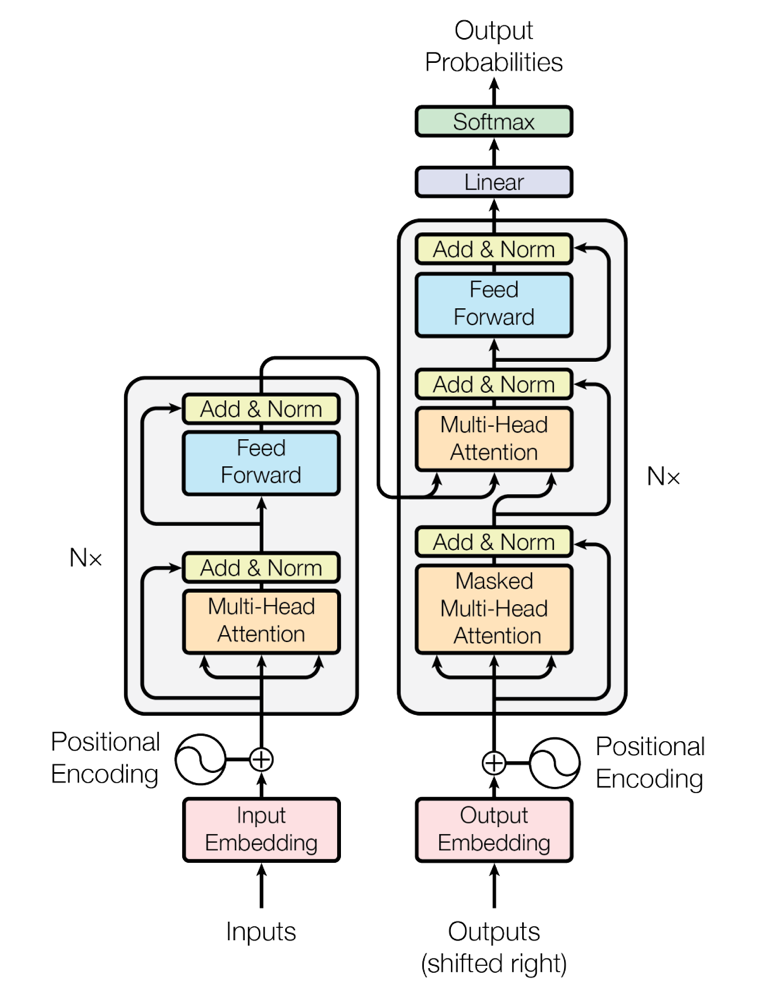
\includegraphics[width=\linewidth]{figs/lec3/lec3.01.png}
    \caption{The original Transformer architecture}
  \end{minipage}
  \hfill
  \begin{minipage}{0.5\linewidth}
    \small
    在Original Transformer Architecture中,我们在选择以下方式来构建Architecture
    \begin{itemize}
    \item \textbf{Norm Type}: Post-norm, LayerNorm
    \item \textbf{FFN Type}: ReLU \\
        \[
        \text{FFN}(z_i) = \text{ReLU}(z_i W_1 + b_1) W_2 + b_2
        \]
    \item \textbf{Position Embedding}: sines and cosines \\
    \begin{align*}
     &\mathrm{PE}(pos,\, 2i)   = \sin \Bigl( pos \,/\, 10000^{\,2i / d_{\mathit{model}}} \Bigr)\\
     &\mathrm{PE}(pos,\, 2i+1) = \cos \Bigl( pos \,/\, 10000^{\,2i / d_{\mathit{model}}} \Bigr)
    \end{align*}

    \end{itemize}

  \end{minipage}
\end{figure}

\MarginImageWithNote
  {figs/lec3/lec3.02.png}
  {\captionof{figure}{Modern Models' Architecture}}
  {}

而这些有许多变体,接下来我们会逐一介绍:
\begin{itemize}
    \item Pre-norm vs. Post-norm
    \item LayerNorm vs. RMSNorm
    \item ReLU, GeLU, *GLU, SwiGLU
    \item Serial vs. Parallel layers
    \item Relative Position Embeddings vs. Absolute Position Embeddings
\end{itemize}

\clearpage
\subsection{Normalization Variants}~{}

\MarginImage
  {figs/lec3/lec3.03.png}
  {\captionof{figure}{Pre-norm vs. Post-norm in residual flow}
  \label{fig:fig3.3}}


\subsubsection{Pre-norm vs. Post-norm in Transformer}~{}

\begin{figure}[htbp]
  \centering
  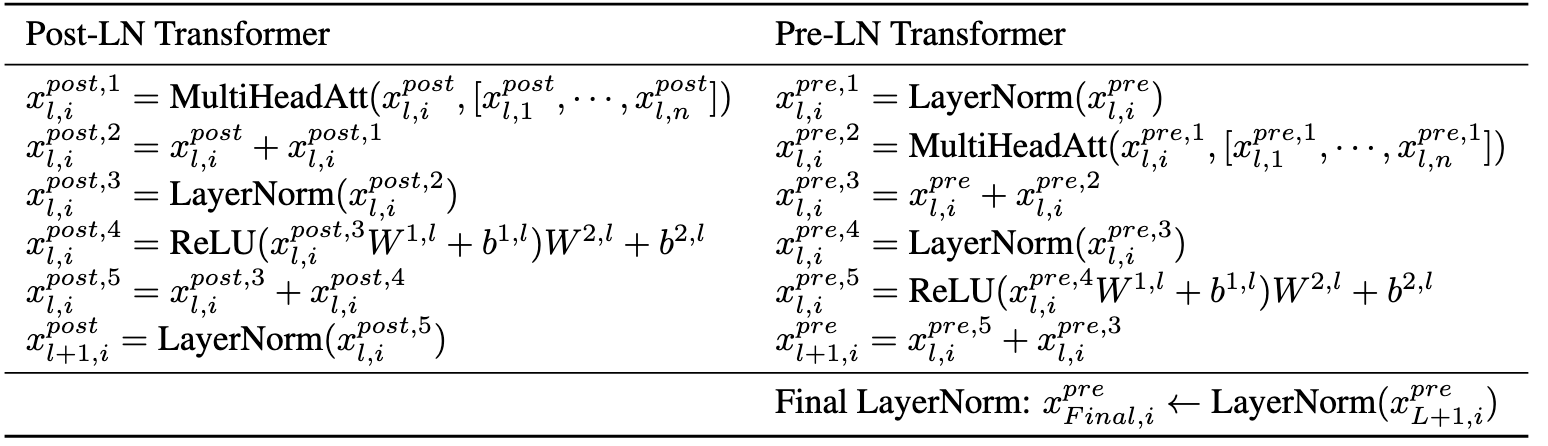
\includegraphics[width=1\linewidth]{figs/lec3/lec3.04.png}
  \captionof{figure}{Post-LN Transformer v.s. Pre-LN Transformer}
  \label{fig:}
\end{figure}

如Figure~\ref{fig:fig3.3}所示,Post-LN 将 LayerNorm 放置在residual signal path 之中,在残差连接之后;而 Pre-LN 将其置于子层输入之前,不置于residual signal path之中。

在论文\textit{On Layer Normalization in the Transformer Architecture}中,作者比较了 Pre-LN 与 Post-LN 的差异,发现 Post-LN 在深层网络中容易出现梯度消失或训练不稳定的问题,
而 Pre-LN 则能够:

\begin{itemize}
  \item Remove warm-up stage
  \item 缓解梯度爆炸与消失问题  
  \item Stability and larger LRs for large networks
\end{itemize}

\paragraph{1. Pre-LayerNorm 可以去除模型对于warm-up阶段的依赖}~{}
\MarginNote{
\Definition{Learning Rate Warm-up Stage}{
Post-LN Transformer 需要先从较小的学习率逐步升高,才能避免训练不稳定
(Popel \& Bojar, 2018)。  

设第 $t$ 次迭代的学习率为 $lr(t)$,训练过程中的最大学习率为 $lr_{\max}$,
给定 warm-up 时间步长 $T_{\text{warm-up}}$,其调度方式为:
\[
lr(t) = \frac{t}{T_{\text{warm-up}}} \, lr_{\max}, \quad t \leq T_{\text{warm-up}}.
\]

在 warm-up 阶段之后,学习率由经典调度器设定,如线性衰减、
逆平方根衰减或特定迭代点的强制衰减(Vaswani et al., 2018)。
}
}

In Figure~\ref{fig:lec3.05}, the x-axis is the epoch number and the y-axis is the BLEU score/validation loss. "w/o warm-up" indicates “without the warm-up stage” while "w/ warm-up" indicates “with the warm-up stage”.\\
In conclusion:
\begin{itemize}
  \item The learning rate warm-up stage is essential for Post-LN Transformer.
  \item The optimization process is sensitive to the value of $T_{\text{warm-up}}$ demanding fine-tuning.
\end{itemize}

这会有两个弊端:
\begin{itemize}
  \item Its configuration significantly affects the final performance. The practitioners need a careful hyper-parameter tuning, which is computationally expensive for large-scale NLP tasks.
  \item The warm-up stage could slow down the optimization. Standard optimization algorithms usually start with a large learning rate for fast convergence. However, when using the warm-up stage, the learning rate has to gradually increase from zero, which may make the training inefficient.
\end{itemize}

  
\MarginImageWithNote
{figs/lec3/lec3.05.png}
{\captionof{figure}{Performance of the models with different learning rate and $T_{\text{warm-up}}$}
  \label{fig:lec3.05}
}

\clearpage
当采取Pre-LayerNorm 后,我们可以安全地去除warm-up阶段的依赖。
\begin{figure}[htbp]
  \centering
  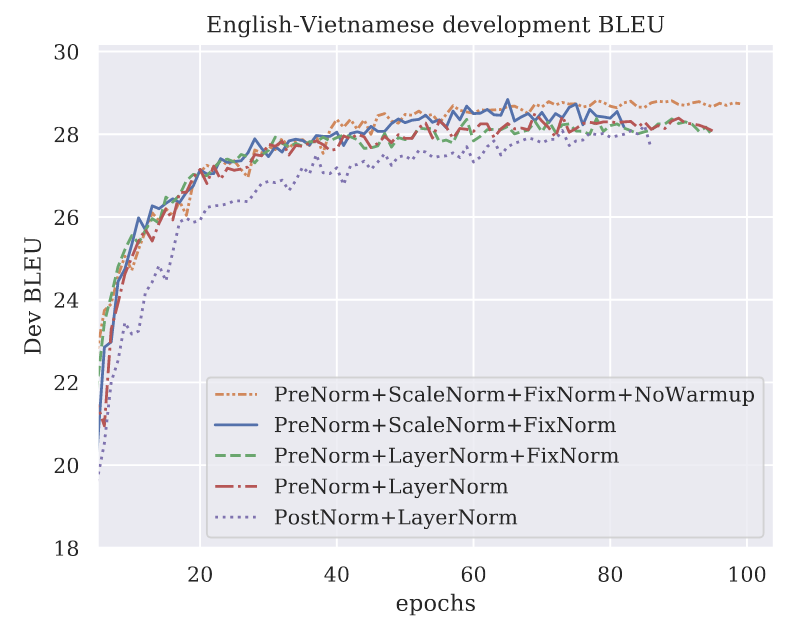
\includegraphics[width=0.8\linewidth]{figs/lec3/lec3.07.png}
  \captionof{figure}{Development BLEU on en→vi with POSTNORM or PRENORM, and with LAYERNORM or SCALENORM.}
\end{figure}

\Proposition{Pre-LayerNorm removes the need for warm-up.}{
Consider a Transformer block with input $\mathbf{x}$, sub-layer function $\mathcal{F}$, and normalization $\text{LN}(\cdot)$.  

\textbf{Post-LN Formulation:}
\[
\mathbf{y} = \text{LN}\big(\mathbf{x} + \mathcal{F}(\mathbf{x})\big).
\]
Backward gradient:
\[
\nabla_{\mathbf{x}} \mathcal{L} = \nabla_{\mathbf{y}}\mathcal{L} \cdot 
\Big( I + J_{\mathcal{F}}(\mathbf{x}) \Big) \cdot J_{\text{LN}}(\mathbf{x}+\mathcal{F}(\mathbf{x})),
\]
where $J$ denotes the Jacobian.  
Since $\text{LN}$ is applied \emph{after} the residual addition, its Jacobian $J_{\text{LN}}$ couples all components, making $\nabla_{\mathbf{x}}$ scale-sensitive.  
A large learning rate can lead to unstable updates $\|\nabla_{\mathbf{x}}\| \gg 1$, hence requiring a warm-up to gradually increase $\eta$.

\textbf{Pre-LN Formulation:}
\[
\mathbf{y} = \mathbf{x} + \mathcal{F}(\text{LN}(\mathbf{x})).
\]
Backward gradient:
\[
\nabla_{\mathbf{x}} \mathcal{L} = \nabla_{\mathbf{y}}\mathcal{L} \cdot 
\Big(I + J_{\mathcal{F}}(\text{LN}(\mathbf{x})) \cdot J_{\text{LN}}(\mathbf{x}) \Big).
\]
Here, normalization is applied \emph{before} the sub-layer.  
Thus the input to $\mathcal{F}$ is always scale-invariant, and the residual path contributes an identity map.  
Therefore the gradient is stabilized around the identity, avoiding exploding/vanishing norms.  

\[
\implies \text{Pre-LN ensures stable optimization, even without warm-up.}
\]
}




\clearpage
\paragraph{2. Pre-LayerNorm 可以缓解梯度爆炸问题}~{}
\\
\begin{figure}[htbp]
  \centering
  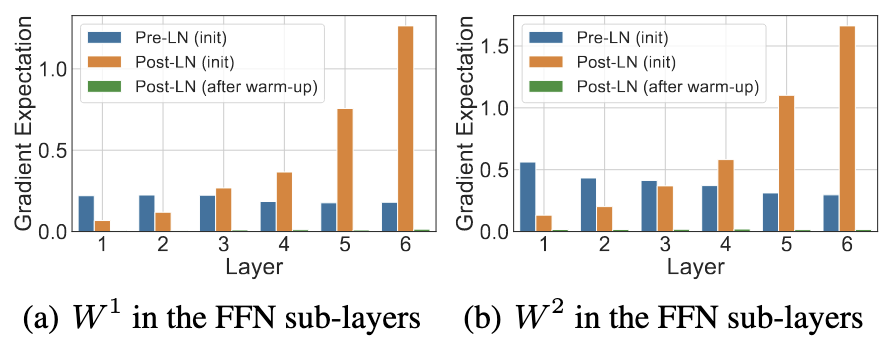
\includegraphics[width=0.65\linewidth]{figs/lec3/lec3.06.png}
  \captionof{figure}{Gradient Attenuation by Pre-LN}
\end{figure}


\begin{figure}[htbp]
  \centering
  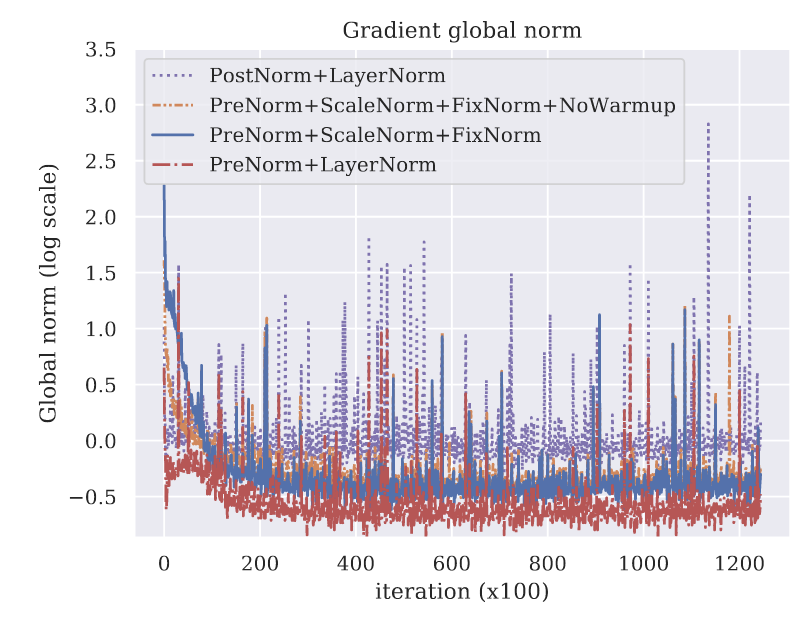
\includegraphics[width=0.65\linewidth]{figs/lec3/lec3.08.png}
  \captionof{figure}{Gradient Spikes}
\end{figure}

\paragraph{3. Pre-LayerNorm 可以提高整体的稳定性并提高Learning Rate加速收敛}~{}
\begin{figure}[htbp]
  \centering
  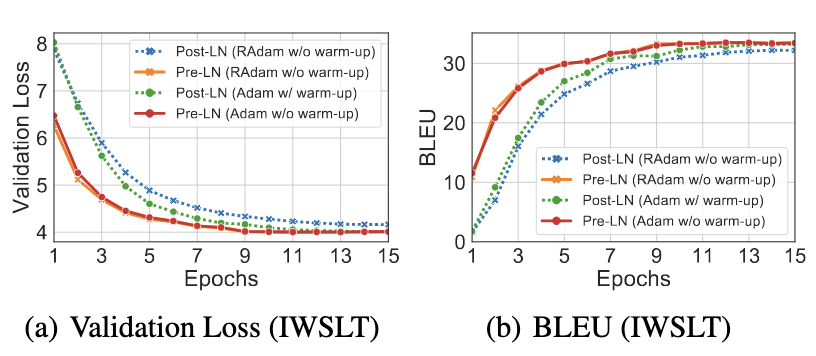
\includegraphics[width=0.65\linewidth]{figs/lec3/lec3.09.png}
  \captionof{figure}{Performances of the models with pre-norm or post-norm}
\end{figure}

\textbf{Almost all modern LMs use pre-norm (but BERT was post-norm)}

\clearpage
\subsubsection{Double Norm}

\begin{figure}[htbp]
  \centering
  \begin{minipage}{0.45\linewidth}
    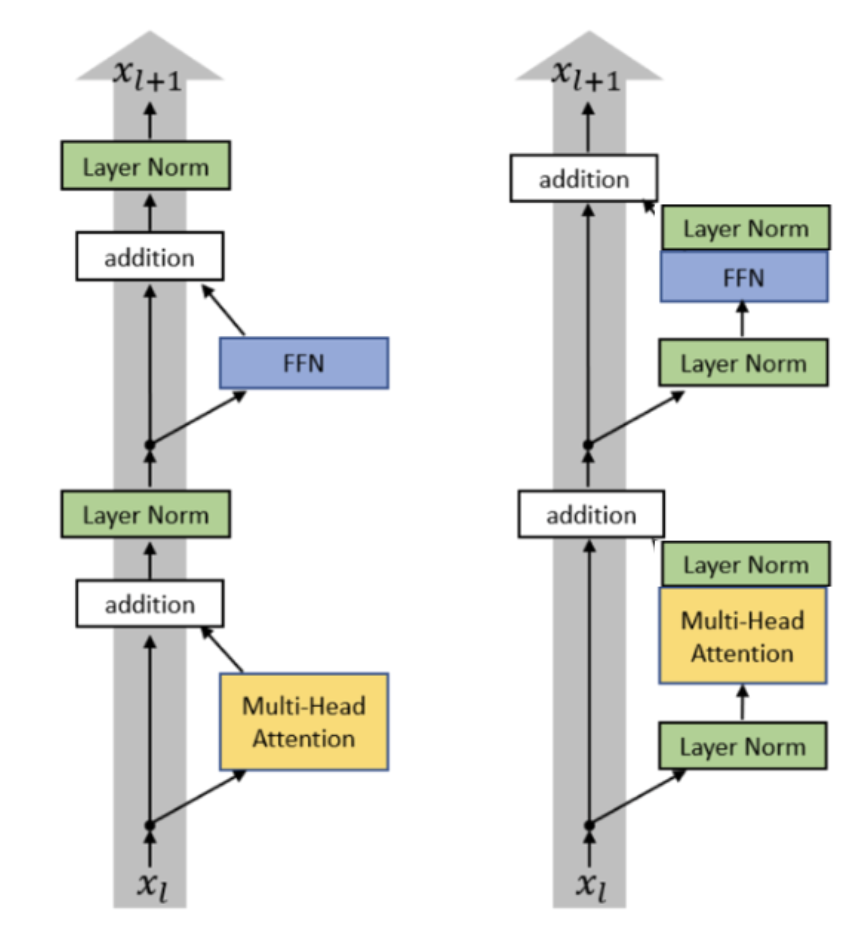
\includegraphics[width=\linewidth]{figs/lec3/lec3.10.png}
    \caption{Transformer with double layernorm }
  \end{minipage}
  \hfill
  \begin{minipage}{0.5\linewidth}
    \small
    \QA
    {Why putting LayerNorms in residual streams is bad?}
    {
    Residual connections provide an identity mapping from lower to higher layers, which is crucial for stable gradient flow in very deep networks.  
    If a LayerNorm is inserted \emph{inside} the residual stream, this identity path is no longer preserved---it is transformed by the normalization operator.  
    As a result, the gradients are no longer guaranteed to propagate cleanly, which can lead to training instability.  
    }
  \end{minipage}
\end{figure}

\textbf{Motivation.}
\begin{itemize}
  \item \emph{Post-LN:} $\mathbf{x}_{l+1} = \text{LN}(\mathbf{x}_l + \mathcal{F}(\mathbf{x}_l))$  
        stabilizes layer-wise distributions but destroys the identity mapping in the residual path, \textbf{leading to unstable gradients and requiring warm-up}.
  \item \emph{Pre-LN:} $\mathbf{x}_{l+1} = \mathbf{x}_l + \mathcal{F}(\text{LN}(\mathbf{x}_l))$  
        preserves the residual identity for stable gradients without warm-up, but lacks normalization after the residual addition, \textbf{causing distribution shift in deep networks}.
\end{itemize}

\textbf{Effect }Double LayerNorm combines the strengths of both: \\ 
\begin{itemize}
  \item \textbf{Norm-in} ($\text{LN}_{\text{in}}$) ensures the input to $\mathcal{F}$ is scale-invariant, preserving stable gradient flow as in Pre-LN.
  \item \textbf{Norm-out} ($\text{LN}_{\text{out}}$) normalizes the residual sum, aligning the output distribution across layers as in Post-LN.
\end{itemize}

Thus, Double LayerNorm avoids the dependency on warm-up while also preventing distribution drift, leading to more stable and scalable training of deep Transformers.

\textbf{Recent Models:} Grok,Gemma 2.



\clearpage
\subsubsection{LayerNorm vs. RMSNorm}

\Definition{Layer Normalization (LayerNorm)}{
给定输入向量 $\mathbf{x} = (x_1, x_2, \dots, x_d) \in \mathbb{R}^d$,LayerNorm 对整个维度做归一化:
\[
\hat{x}_i = \frac{x_i - \mu}{\sqrt{\sigma^2 + \epsilon}}, 
\quad \mu = \frac{1}{d}\sum_{j=1}^d x_j, 
\quad \sigma^2 = \frac{1}{d}\sum_{j=1}^d (x_j - \mu)^2.
\]
最后再进行可学习($\gamma$, $\beta$)的仿射变换:
\[
y_i = \gamma \hat{x}_i + \beta, \quad \gamma, \beta \in \mathbb{R}^d.
\]
它显式地移除了均值并缩放方差,保证归一化后的特征分布具有零均值和单位方差。

\textbf{Notable models:} GPT3/2/1, OPT, GPT-J
}

\Definition{Root Mean Square Normalization (RMSNorm)}{
RMSNorm 省略了均值归一化,仅基于均方根 (RMS) 对输入缩放:
\[
\hat{x}_i = \frac{x_i}{\sqrt{\frac{1}{d}\sum_{j=1}^d x_j^2 + \epsilon}},
\]
再施加可学习的缩放参数($\gamma$):
\[
y_i = \gamma \hat{x}_i, \quad \gamma \in \mathbb{R}^d.
\]
RMSNorm 保持输入方向不变,仅依赖整体幅值的缩放。
\textbf{Notable models:} LLaMA-family, PaLM, Chinchilla
}

\QA{Why RMSNorm?}
{
\begin{itemize}
  \item \textbf{Fewer operations} No mean calculation
  \item \textbf{Fewer parameters} No bias term to store
\end{itemize}
}


\MarginImageWithNote
{figs/lec3/lec3.11.png}
{\captionof{figure}{Proportion of FLOPs across different operations}}
{\textbf{Matrix multipliers are the \textit{vast majority of FLOPs (and memory)}}}

\MarginImageWithNote
{figs/lec3/lec3.12.png}
{\captionof{figure}{Proportion of Runtime across different operations}}
{\textbf{RMSNorm can still matter due to the importance \textit{data movement.}}}

\Remark{
\textbf{  FLOPS are not runtime!
}}

\MarginImageWithNote
{figs/lec3/lec3.13.png}
{\captionof{figure}{FLOPS and FLOP-to-memory ratio in Transformer}}

\begin{figure}[htbp]
  \centering
  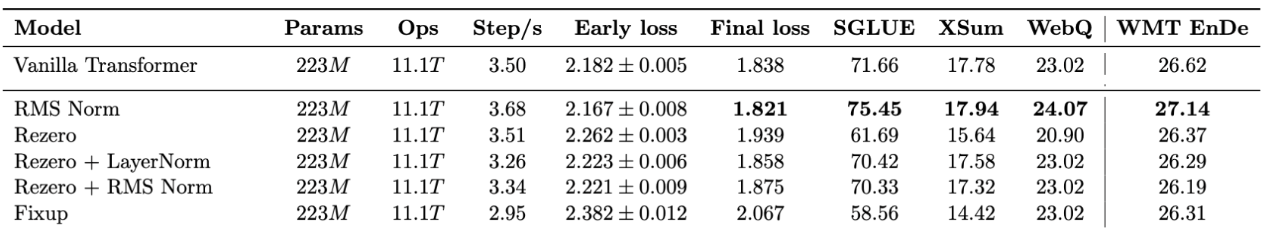
\includegraphics[width=0.8\linewidth]{figs/lec3/lec3.14.png}
  \captionof{figure}{RMSNorm runtime}
\end{figure}

\Insight{Dropping Bias Terms}{
Most modern Transformers omit explicit bias terms.  

\textbf{Original Transformer (Vaswani et al., 2017):}
\[
\text{FFN}(x) = \max\!\bigl(0,\, xW_1 + b_1\bigr)W_2 + b_2
\]

\textbf{Typical Modern Implementation (non-gated):}
\[
\text{FFN}(x) = \sigma(xW_1)W_2
\]

\textbf{Reasons:}  
{\color{dblue}{
- \emph{Memory efficiency:} Similar to RMSNorm, removing biases reduces parameter count and memory footprint.  \\
- \emph{Optimization stability:} Empirically, biases contribute little to training stability in deep architectures, so omitting them avoids redundant parameters.  
}}
}

\clearpage
\subsection{Activation Variants}
\paragraph{A few of the common activations}~{}

\MarginImageWithNote
  {figs/lec3/lec3.15.png}
  {\captionof{figure}{ReLU vs. GELU}}
  {ReLU is flat  for $x<0$, while GELU provides a smoother transition with a small bump around the origin.}

% ---------- 非门控 FFN:与论文一致的无偏置写法 ----------
\begin{itemize}
  \item \textbf{ReLU (Rectified Linear Unit):}
  \begin{align*}
    \mathrm{ReLU}(z) &= \max(0, z), \\
    \mathrm{FFN}_{\mathrm{ReLU}}(x, W_1, W_2, b_1, b_2) 
      &= \max(0,\, xW_1+b_1)\,W_2 + b_2.
    \tag{3.1}
  \end{align*}

  \item \textbf{GELU (Gaussian Error Linear Unit):}
  \begin{align*}
    \mathrm{GELU}(z) &= z \cdot \Phi(z) \\
                     &= \frac{z}{2}\Bigl(1+\mathrm{erf}\!\left(\tfrac{z}{\sqrt{2}}\right)\Bigr), \\
    \mathrm{FFN}_{\mathrm{GELU}}(x, W_1, W_2, b_1, b_2) 
      &= \mathrm{GELU}(xW_1+b_1)\,W_2 + b_2.
    \tag{3.2}
  \end{align*}
  其中
  \[
  \Phi(z)=\tfrac{1}{2}\Bigl(1+\mathrm{erf}\!\left(\tfrac{z}{\sqrt{2}}\right)\Bigr),
  \quad
  \mathrm{erf}(u)=\tfrac{2}{\sqrt{\pi}}\int_0^u e^{-t^2}\,dt.
  \]
\end{itemize}


\paragraph{Gated activations(*GLU)}~{}

GLU-style activations replace this with a gated version:
\[
  {\color{tred}{\max(0,\,xW_1)}} 
  \;\;\longrightarrow\;\;
  {\color{dblue}{\max(0,\,xW_1)}} \odot (xV),
\]
where $(xV)$ is the gate vector applied entrywise.

\Definition{Entrywise (Hadamard) Product $\odot$}{
Given two vectors $\mathbf{a}, \mathbf{b} \in \mathbb{R}^d$, their entrywise (Hadamard, element-wise) product is
\[
(\mathbf{a} \odot \mathbf{b})_i = a_i \, b_i, \quad i=1,\dots,d.
\]
In gated feed-forward networks (GLU and its variants), one branch generates the main signal while the other generates a gate vector; the Hadamard product $\odot$ applies the gate to each dimension individually.
}

\MarginImageWithNote
{figs/lec3/lec3.16.png}
{\captionof{figure}{GLUE Language-Understanding Benchmark}}
{
\textbf{Swish$_1$ vs. Swish$_\beta$}\\[0.3em]
一般形式:$\mathrm{Swish}_\beta(x)=x\sigma(\beta x)$.\\
- $\beta=1$ 固定时 $\Rightarrow$ Swish$_1$.\\
- $\beta$ 可调时 $\Rightarrow$ Swish$_\beta$, 曲线形状可随 $\beta$ 改变:$\beta\to0$ 近似线性,$\beta\to\infty$ 接近 ReLU.
}

\begin{itemize}
  \item \textbf{ReGLU (ReLU Gated Linear Unit):}
  \begin{align*}
    \mathrm{ReGLU}(x) &= \max(0,\, xW_1) \odot (xV), \\
    \mathrm{FFN}(x)   &= \mathrm{ReGLU}(x)W_2.
  \end{align*}
  其中第一项是 ReLU 激活后的主分支,第二项 $(xV)$ 作为门控向量,两者做 Hadamard product。

  \item \textbf{GeGLU (GELU Gated Linear Unit):}
  \begin{align*}
    \mathrm{GeGLU}(x) &= \mathrm{GELU}(xW_1) \odot (xV), \\
    \mathrm{FFN}(x)   &= \mathrm{GeGLU}(x)W_2.
  \end{align*}
  将 ReLU 换成 GELU,使得门控更平滑,广泛用于 GPT-3、PaLM 等大模型。

  \item \textbf{SwiGLU (Swish Gated Linear Unit):}
  \begin{align*}
    \mathrm{SwiGLU}(x) &= \mathrm{Swish_1}(xW_1) \odot (xV), \\
    \mathrm{FFN}(x)    &= \mathrm{SwiGLU}(x)W_2,
  \end{align*}
\end{itemize}




\clearpage
\subsection{Serial vs. Parallel layers}

\MarginNote{
\QA{Why faster?}{
In parallel blocks, both Attention and MLP take the same $\mathrm{LN}(x)$ as input. \\
$\Rightarrow$ Their input projections can be \textit{fused} into a single large matmul: 
\[
[xW_Q,\, xW_K,\, xW_V,\, xW_1] = x \cdot W
\] 
instead of separate ones.\\
This reduces GPU kernel launches \& memory traffic, yielding about \textbf{15\% speedup} at large scale.
} 
\textbf{Recent Models:} Cohere Command A, Falcon 2 11B, Command R+
}


\begin{figure}[htbp]
  \centering
  \begin{minipage}{0.45\linewidth}
    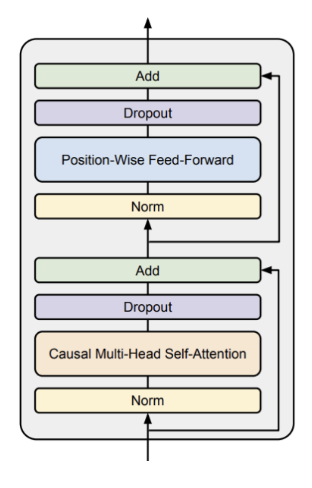
\includegraphics[width=\linewidth]{figs/lec3/lec3.17.png}
    \caption{A transformer block in original transformer}
  \end{minipage}
  \hfill
  \begin{minipage}{0.5\linewidth}
    \small
      Normal Transformer blocks are \textit{serial}: they compute attention, then the MLP. \\
      Now a few models (e.g., GPT-J, PaLM, GPT-NeoX) adopt \textit{parallel layers}. \\
      \textbf{Serial formulation (standard):}  \\
      \[
        y = x + \mathrm{MLP}\bigl(\mathrm{LN}(x + \mathrm{Attention}(\mathrm{LN}(x)))\bigr)
      \]
      \textbf{Parallel formulation:}
      \[
        y = x + \mathrm{MLP}(\mathrm{LN}(x)) + \mathrm{Attention}(\mathrm{LN}(x))
      \]

      Parallel formulation allows the MLP and Attention input projections to be computed together, giving about 
      \textbf{15\% faster training at large scale}. \\ 
      Empirically, PaLM observed \textit{no quality degradation at 62B scale}, so the effect is considered quality-neutral at 540B.
  \end{minipage}
\end{figure}


\clearpage
\subsection{RoPE: Rotary Position Embeddings}

\paragraph{A few of commom embeddings}~{}
\\
\MarginNote{
Recall: For a token $x$ at position $i$: 
\[
\mathrm{Embed}(x,i) = v_x + \mathrm{PE}_i
\]
}

\begin{itemize}
  \item \textbf{Sine embeddings:} add sines and cosines that enable localization
  \begin{align*}
    \mathrm{PE}_{(pos,2i)}   &= \sin\!\left(\frac{pos}{10000^{2i/d_{\text{model}}}}\right), \\
    \mathrm{PE}_{(pos,2i+1)} &= \cos\!\left(\frac{pos}{10000^{2i/d_{\text{model}}}}\right),
  \end{align*}
  where $pos$ is the position index, $i$ is the dimension index.

\item \textbf{Absolute embeddings:} add a position vector to the embedding
  \begin{align*}
    \mathrm{Embed}(x,i) &= v_x + u_i
  \end{align*}
  where 
  \begin{itemize}
    \item $v_x \in \mathbb{R}^{d_z}$ : token $x$ 的词向量 (word embedding),
    \item $u_i \in \mathbb{R}^{d_z}$ : 位置 $i$ 的绝对位置向量 (absolute positional embedding)。
  \end{itemize}

  \item \textbf{Relative embeddings:} add a bias term to the \textit{attention computation}
  \begin{align*}
    e_{ij} &= \frac{x_i W^Q \,(x_j W^K + {\color{tred}a_{ij}^K)}^T}{\sqrt{d_z}}
  \end{align*}
  where
  \begin{itemize}
    \item $x_i \in \mathbb{R}^{d_z}$ : 第 $i$ 个位置的输入表示,
    \item $W^Q, W^K \in \mathbb{R}^{d_z \times d_z}$ : query 与 key 的投影矩阵,
    \item $x_i W^Q$ : 位置 $i$ 的 query 向量,
    \item $x_j W^K$ : 位置 $j$ 的 key 向量,
    \item {\color{tred}$a_{ij}^K$} $\in  \mathbb{R}^{d_z}$ : 与相对距离 $(i-j)$ 相关的相对位置嵌入,
    \item 分母 $\sqrt{d_z}$ : 标准 attention 中的缩放因子。
  \end{itemize}
  Thus, $e_{ij}$ is the attention score between position $i$ and $j$, augmented with relative positional information.
\end{itemize}

\paragraph{High level thought process: Relativity }~{}
\\
\Remark{
A \textbf{relative position embedding} should be a mapping $f(x,i)$ such that
\[
\langle f(x,i), f(y,j) \rangle \;=\; g(x,y,\, i-j).
\]
That is, the attention score depends not only on the content $(x,y)$, 
but also only on the \textit{relative position} $(i-j)$, rather than the absolute indices $i$ or $j$.
}

How do existing embeddings not fulfill this goal?

\begin{itemize}
  \item \textbf{Sine:} Has various cross-terms that are not purely relative. 
  \[
    \langle \mathrm{Embed}(x,i), \mathrm{Embed}(y,j) \rangle 
      = \langle v_x, v_y \rangle 
      + \langle \mathrm{PE}_i, v_y \rangle + \cdots
  \]
  So the score depends on both token embeddings and absolute position terms.

  \item \textbf{Absolute:} Obviously not relative --- embeddings $u_i$ are tied to absolute positions $i$ rather than $(i-j)$.

  \item \textbf{Relative embeddings:} 
  \[
    e_{ij} = \frac{x_i W^Q (x_j W^K + a_{ij}^K)^T}{\sqrt{d_z}}
  \]
  encodes relative information, but this modification is no longer a \textbf{pure inner product} between query and key; it adds an extra bias term. 
\end{itemize}

\paragraph{RoPE: rotary position embeddings}~{}
\QA{How can we solve this problem?}
{
\begin{itemize}
  \item Our embeddings should be invariant to absolute positions.
  \item The inner products are invariante to arbitrary rotations.
\end{itemize}
}

\subsubsection*{A 2D case}

\MarginNote{
  \Definition{Euler's Formula}{
    在复数平面上,$e^{i\theta} = \cos\theta + i\sin\theta$。
    乘上 $e^{i\theta}$ 相当于把二维向量旋转角度 $\theta$:
    \begin{align*}
      (a+ib)\,e^{i\theta}
      &= (a\cos\theta - b\sin\theta) \\
      &+ i(a\sin\theta + b\cos\theta).
    \end{align*}
    因此,复数乘以 $e^{i\theta}$ 本质上就是一个二维旋转。
  }
}   


在二维情况下,我们可以把词向量 $\mathbf{x}_m$ 经过线性变换 $\mathbf{W}_q$ 或 $\mathbf{W}_k$ 后,
再乘上一个旋转因子 $e^{i m \theta}$ 或 $e^{i n \theta}$,分别得到

\begin{align*}
f_q(\mathbf{x}_m,m) &= (\mathbf{W}_q \mathbf{x}_m) e^{i m \theta},\\
f_k(\mathbf{x}_n,n) &= (\mathbf{W}_k \mathbf{x}_n) e^{i n \theta}.\\
g(\mathbf{x}_m,\mathbf{x}_n,m-n) 
&= \operatorname{Re}\!\left[(\mathbf{W}_q \mathbf{x}_m)(\mathbf{W}_k \mathbf{x}_n)^{*} e^{i (m-n)\theta}\right],
\end{align*}

其中 $(\cdot)^*$ 表示共轭复数,$\operatorname{Re}[\cdot]$ 取实部。
这个形式表明:打分结果只依赖位置差 $(m-n)$,从而实现了相对位置编码。

进一步地,$f_q$ 也可以写成矩阵形式:
\begin{align*}
f_{q}(\mathbf{x}_m, m) &=
\begin{pmatrix}
\cos(m\theta) & -\sin(m\theta) \\
\sin(m\theta) &  \cos(m\theta)
\end{pmatrix}
\begin{pmatrix}
W^{(11)}_q & W^{(12)}_q \\
W^{(21)}_q & W^{(22)}_q
\end{pmatrix}
\begin{pmatrix}
x^{(1)}_m \\
x^{(2)}_m
\end{pmatrix}.\\
&=
\begin{pmatrix}
\cos(m\theta) & -\sin(m\theta) \\
\sin(m\theta) &  \cos(m\theta)
\end{pmatrix}
\begin{pmatrix}
q^{(1)}_m \\
q^{(2)}_m
\end{pmatrix}
\end{align*}
看到这里会发现,这不就是 query 向量乘以了一个旋转矩阵吗?这就是为什么叫做旋转位置编码的原因。



同理,$f_k$ 也可以写成矩阵形式:
\begin{align*}
f_{k}(\mathbf{x}_n, n) &=
\begin{pmatrix}
\cos(n\theta) & -\sin(n\theta) \\
\sin(n\theta) &  \cos(n\theta)
\end{pmatrix}
\begin{pmatrix}
W^{(11)}_k & W^{(12)}_k \\
W^{(21)}_k & W^{(22)}_k
\end{pmatrix}
\begin{pmatrix}
x^{(1)}_n \\
x^{(2)}_n
\end{pmatrix}.\\
&=
\begin{pmatrix}
\cos(n\theta) & -\sin(n\theta) \\
\sin(n\theta) &  \cos(n\theta)
\end{pmatrix}
\begin{pmatrix}
k^{(1)}_n \\
k^{(2)}_n
\end{pmatrix}
\end{align*}

这里的 $f_q,f_k$ 可以统一表示为:
\[
f_{\{q, k\}}(\mathbf{x}_m, m) =
\begin{pmatrix}
\cos(m\theta) & -\sin(m\theta) \\
\sin(m\theta) &  \cos(m\theta)
\end{pmatrix}
\begin{pmatrix}
W^{(11)}_{\{q, k\}} & W^{(12)}_{\{q, k\}} \\
W^{(21)}_{\{q, k\}} & W^{(22)}_{\{q, k\}}
\end{pmatrix}
\begin{pmatrix}
x^{(1)}_m \\
x^{(2)}_m
\end{pmatrix}.
\]


最终 $g(\mathbf{x}_m,\mathbf{x}_n,m-n)$ 可以表示如下:
\begin{equation*}
g(\mathbf{x}_m,\mathbf{x}_n,m-n) =
\begin{pmatrix}
q^{(1)}_m & q^{(2)}_m
\end{pmatrix}
\begin{pmatrix}
\cos((m-n)\theta) & -\sin((m-n)\theta) \\
\sin((m-n)\theta) &  \cos((m-n)\theta)
\end{pmatrix}
\begin{pmatrix}
k^{(1)}_n \\
k^{(2)}_n
\end{pmatrix}.
\end{equation*}





直观理解:RoPE 的做法就是“先线性变换,再按照位置索引旋转一个角度”,
这样点积相似度天然包含了相对位置信息。

\begin{figure}[htbp]
  \centering
  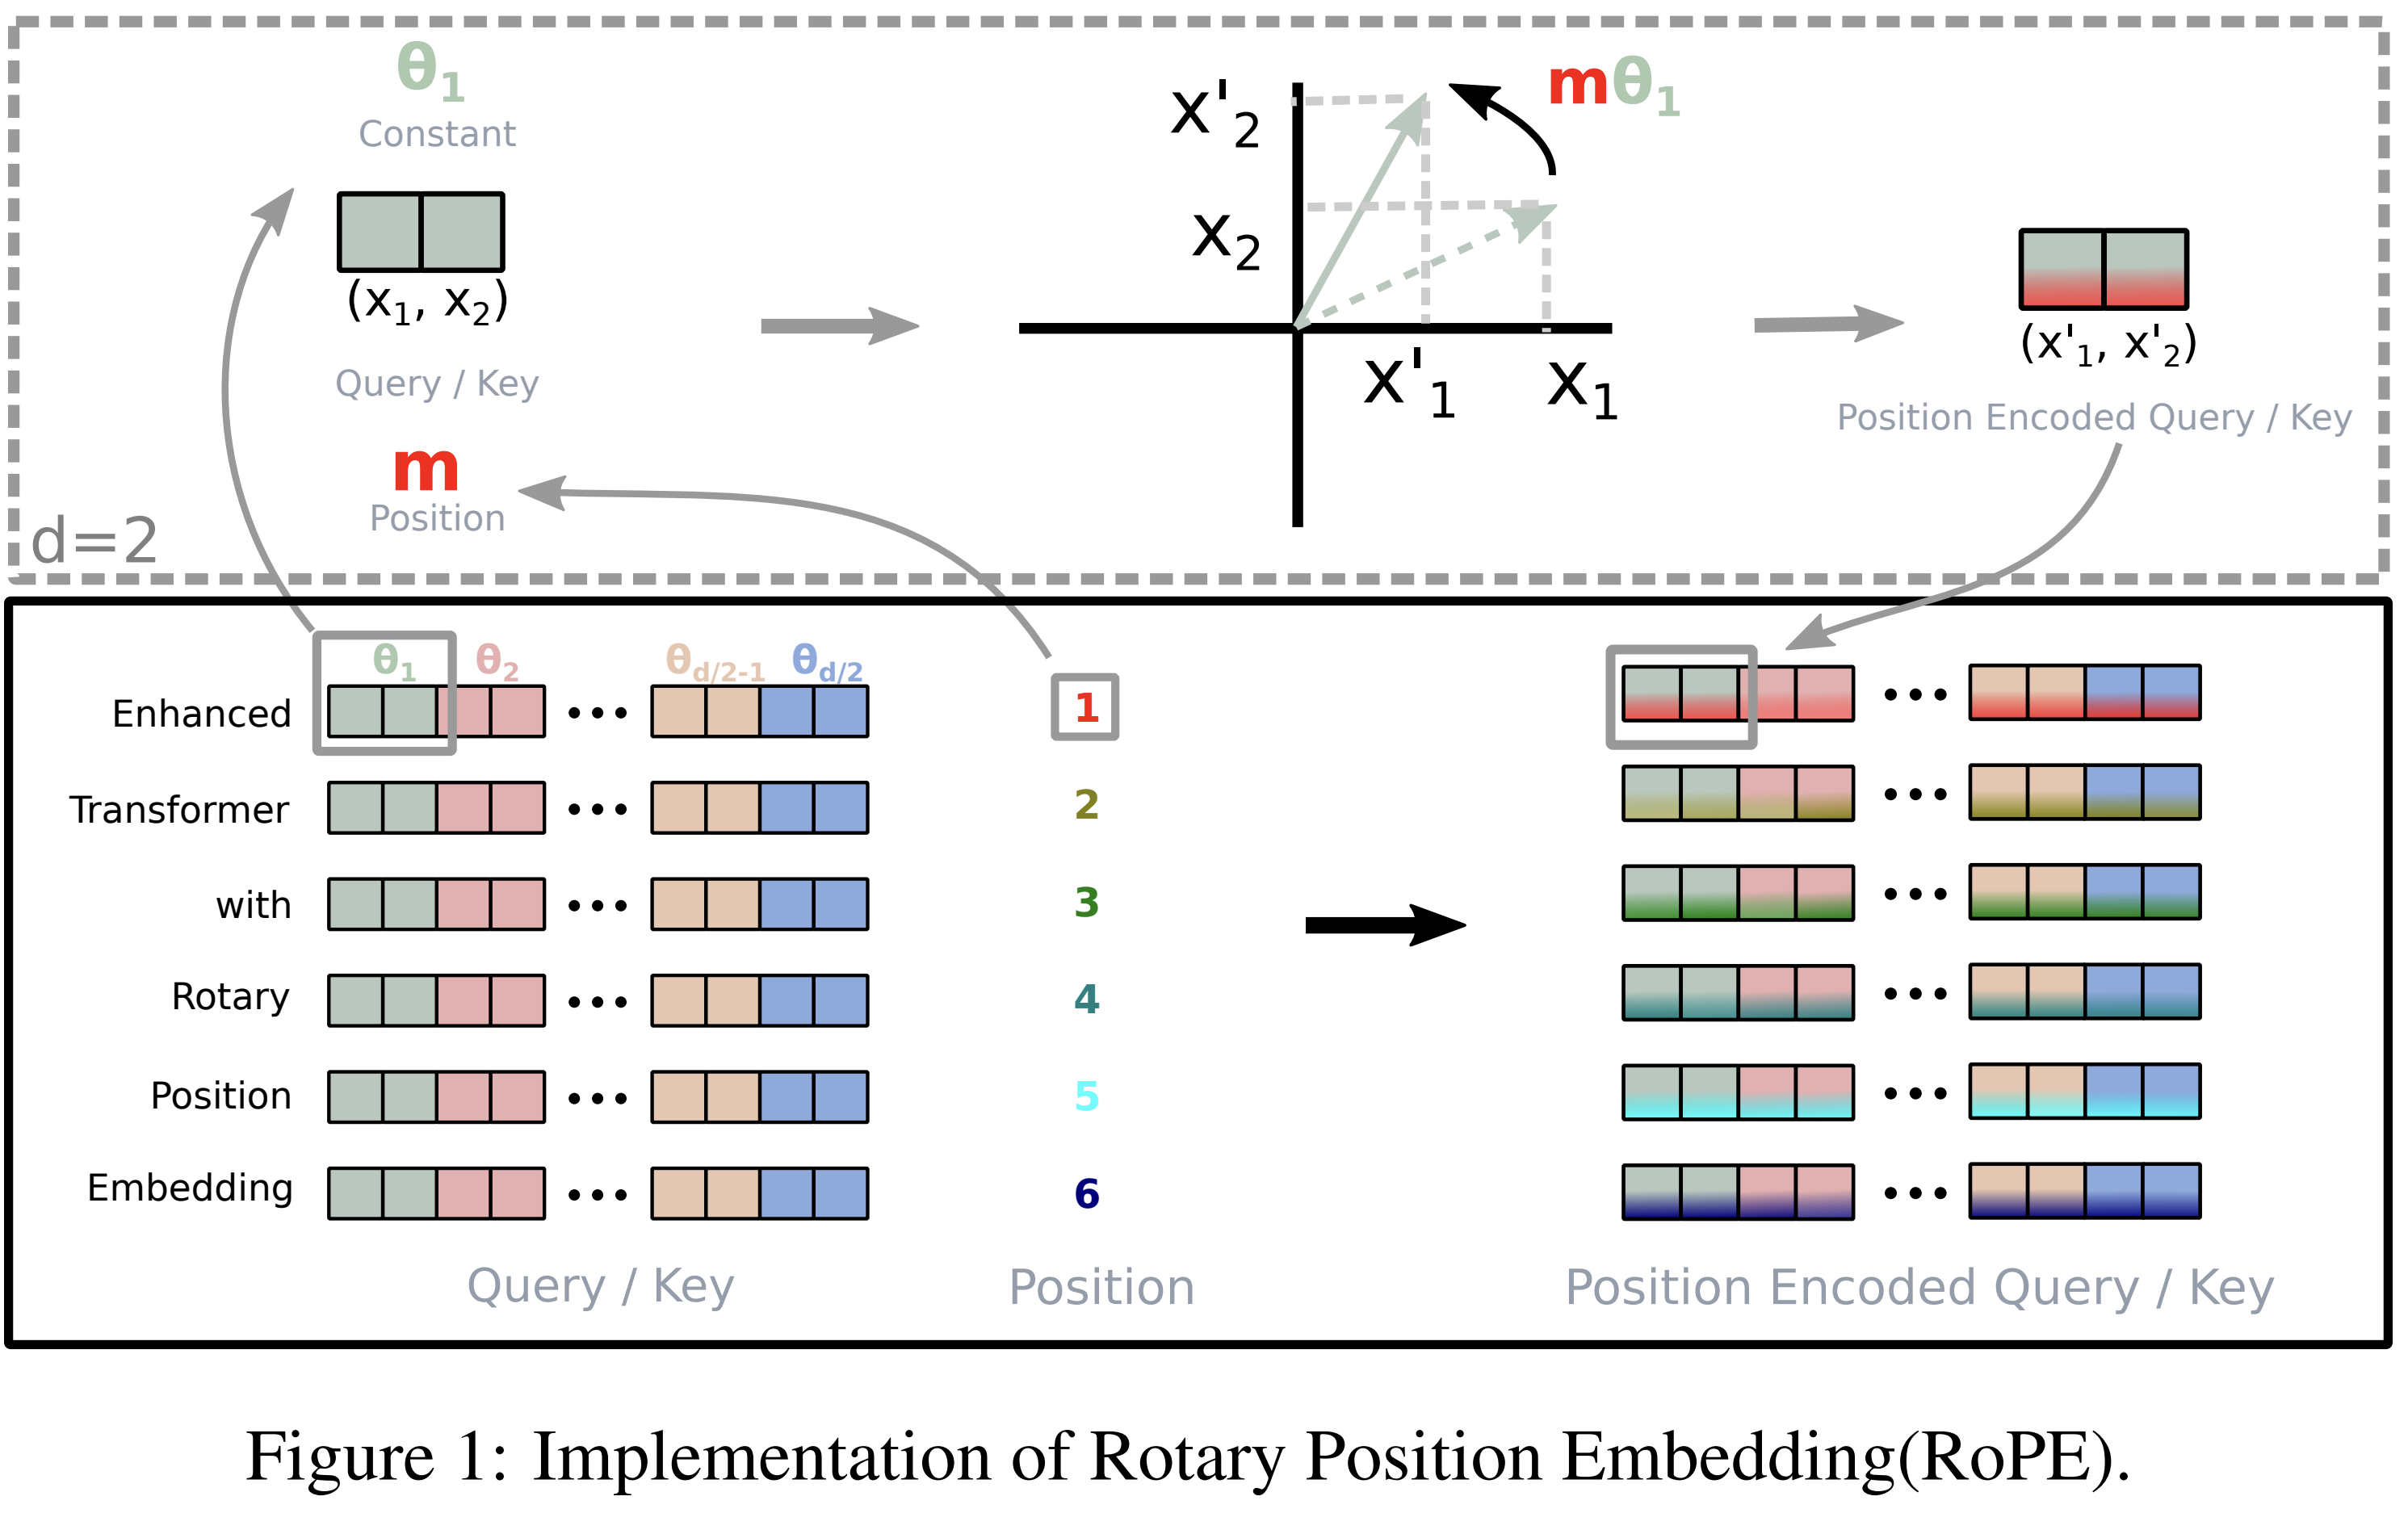
\includegraphics[width=0.8\linewidth]{figs/lec3/lec3.18.png}
  \captionof{figure}{Implementation of Rotary Position Embedding(RoPE).}
\end{figure}


\subsubsection{General form}~{}

从二维情况出发,我们希望推广到任意偶数维度 $d$。设 $\mathbf{x}_i \in \mathbb{R}^d$,我们将 $d$ 维空间划分为 $d/2$ 个二维子空间,并在每个子空间内独立应用二维旋转。利用内积的线性性,可以将 $f_{\{q, k\}}$ 统一写作:
\begin{equation*}
	f_{\{q, k\}}(\mathbf{x}_m, m) 
	= \mathbf{R}^d_{\Theta, m}\,\mathbf{W}_{\{q, k\}}\,\mathbf{x}_m,
	\label{fn:rope-fqk}
\end{equation*}
其中 $\mathbf{R}^d_{\Theta,m}$ 是 $d\times d$ 的分块对角旋转矩阵:
\begin{equation*}    
	\mathbf{R}^d_{\Theta,m} = 
	\begin{pmatrix}
		\cos(m\theta_1)& -\sin(m\theta_1)&0&0&\cdots&0&0\\
		\sin(m\theta_1)& \cos(m\theta_1)&0&0&\cdots&0&0 \\
		0&0&\cos(m\theta_2)& -\sin(m\theta_2)&\cdots&0&0\\
		0&0&\sin(m\theta_2)& \cos(m\theta_2)&\cdots&0&0 \\
		\vdots&\vdots&\vdots&\vdots&\ddots&\vdots&\vdots\\
		0&0&0&0&\cdots&\cos(m\theta_{d/2})& -\sin(m\theta_{d/2})\\
		0&0&0&0&\cdots&\sin(m\theta_{d/2})& \cos(m\theta_{d/2})
	\end{pmatrix},
	\label{fn:rope-RMat}
\end{equation*}

其中参数集合为
\[
\Theta = \Bigl\{\,\theta_i = 10000^{-\tfrac{2(i-1)}{d}},\; i=1,2,\dots,d/2\Bigr\}.
\]

这种结构本质上就是在每个二维子空间内进行旋转,并通过分块对角的拼接推广到 $d$ 维。

\vspace{0.5em}
将 RoPE 应用于自注意力机制,有:
\begin{equation}
	\mathbf{q}_m^{\top}\mathbf{k}_n
	= \bigl(\mathbf{R}^d_{\Theta, m}\mathbf{W}_q\mathbf{x}_m\bigr)^{\!\top}
	\bigl(\mathbf{R}^d_{\Theta, n}\mathbf{W}_k\mathbf{x}_n\bigr)
	= \mathbf{x}_m^{\top}\mathbf{W}_q^\top \mathbf{R}^d_{\Theta, n-m}\mathbf{W}_k\mathbf{x}_n,
	\label{fn:rope-qk}
\end{equation}
其中
\[
\mathbf{R}^d_{\Theta, n-m} = (\mathbf{R}^d_{\Theta, m})^\top \mathbf{R}^d_{\Theta, n}.
\]

需要注意的是,$\mathbf{R}^d_{\Theta,m}$ 是正交矩阵,保证了在引入位置编码时不会破坏数值稳定性。另外,由于 $\mathbf{R}^d_{\Theta}$ 的稀疏分块结构,直接进行矩阵乘法并不高效;在实际实现中通常采用对偶维度成对旋转的写法来避免显式构造整个矩阵。

\subsection{Properties of RoPE}
\label{sec:prop-of-RoPE}

\paragraph{长程衰减 (Long-term decay).} 
在 RoPE 的设计中,我们为每一对维度分配一个频率参数 $\theta_i=10000^{-2i/d}$。  
这样的设置带来一个重要性质:当两个 token 的相对位置差 $(m-n)$ 逐渐增大时,它们的旋转角度差也会逐渐增大,从而使得内积的结果逐渐减小。  
这意味着,随着相对距离变大,query 和 key 之间的相似度会自动衰减,体现了“距离越远,关联越弱”的直觉。  
这一性质保证了 RoPE 在编码长文本时能够自然地控制长程依赖的强度。

\paragraph{结合线性注意力 (RoPE with linear attention).} 
我们知道自注意力机制可以写成一个通用的加权平均形式:
\begin{equation}
	\operatorname{Attention}(\mathbf{Q},\mathbf{K},\mathbf{V})_m
	= \frac{\sum_{n=1}^{N}\operatorname{sim}(\mathbf{q}_m,\mathbf{k}_n)\,\mathbf{v}_n}
	{\sum_{n=1}^{N}\operatorname{sim}(\mathbf{q}_m,\mathbf{k}_n)}.
	\label{fn:atten-full}
\end{equation}

原始的自注意力选择 $\operatorname{sim}(\mathbf{q}_m,\mathbf{k}_n)=\exp(\mathbf{q}_m^\top \mathbf{k}_n / \sqrt{d})$,需要对每一对 $(m,n)$ 计算内积,复杂度是 $\mathcal{O}(N^2)$。  
为了降低计算复杂度,线性注意力提出把相似度函数改写为可分解的形式:

\begin{equation}
	\operatorname{Attention}(\mathbf{Q},\mathbf{K},\mathbf{V})_m
	= \frac{\sum_{n=1}^{N}\phi(\mathbf{q}_m)^\top \varphi(\mathbf{k}_n)\,\mathbf{v}_n}
	{\sum_{n=1}^{N}\phi(\mathbf{q}_m)^\top \varphi(\mathbf{k}_n)},
	\label{fn:linear-attention}
\end{equation}
其中 $\phi(\cdot),\varphi(\cdot)$ 是一些非负函数(例如可以取 $\operatorname{elu}(x)+1$ 或者 softmax)。  
这种改写利用了矩阵乘法的结合律,可以先把 $\varphi(\mathbf{k}_n)\mathbf{v}_n$ 累加,再和 $\phi(\mathbf{q}_m)$ 相乘,从而避免显式计算所有 $\mathcal{O}(N^2)$ 的内积。

\medskip
那么 RoPE 如何与线性注意力结合呢?  
关键在于:RoPE 通过旋转矩阵 $\mathbf{R}^d_{\Theta,m}$ 注入位置信息,而旋转矩阵是正交的,不会改变向量的模长。  
因此我们可以在 $\phi(\mathbf{q}_m)$ 和 $\varphi(\mathbf{k}_n)$ 的输出之后,再乘上旋转矩阵,即:
\begin{equation}
	\operatorname{Attention}(\mathbf{Q},\mathbf{K},\mathbf{V})_m
	= \frac{\sum_{n=1}^{N}\big(\mathbf{R}^d_{\Theta,m}\phi(\mathbf{q}_m)\big)^\top
	\big(\mathbf{R}^d_{\Theta,n}\varphi(\mathbf{k}_n)\big)\,\mathbf{v}_n}
	{\sum_{n=1}^{N}\phi(\mathbf{q}_m)^\top \varphi(\mathbf{k}_n)}.
	\label{fn:linear-rope}
\end{equation}

\paragraph{说明.} 
在这里,分母保持不变,以避免出现除以零的风险。分子部分由于旋转可能引入负值,因此得到的注意力权重并不一定是严格的概率分布。  
但这种形式仍然能正确工作,并且成功地将相对位置信息注入到线性注意力中。

\MarginImageWithNote
{figs/lec3/lec3.19.png}
{\captionof{figure}{Implementation and code for RoPE}}
{\textbf{NOTE:} embedding at \textit{each attention operation} to enforce positive invariance.}


\clearpage
{\chaptoc\noindent\begin{minipage}[inner sep=0,outer sep=0]{0.9\linewidth}\section{Hyperparameters}\end{minipage}}
\\

\subsection{Feedforward Dimension Ratio}











\subsection{Head Dimension and Model Dimension}

\subsection{Aspect Ratio}

\subsection{Vocabulary Size}

\subsection{Regularization}



\clearpage
{\chaptoc\noindent\begin{minipage}[inner sep=0,outer sep=0]{0.9\linewidth}\section{Stability tricks}\end{minipage}}
\\

\subsection{Output Softmax Stability}

\subsection{Attention Softmax Stability}

\subsection{Logit Soft-Capping}



\clearpage
{\chaptoc\noindent\begin{minipage}[inner sep=0,outer sep=0]{0.9\linewidth}\section{Attention Heads}\end{minipage}}
\\

\subsection{Grouped-Query Attention \& Multi-Query Attention}

\subsection{Sparse/Sliding Window Attention}

\subsection{Hybrid Approaches}

% 图 1:OPT FLOPs 构成
% \MarginImageWithNote
%   {figs/}
%   {\captionof{figure}{}}
%   {
%   }

% \begin{figure}[htbp]
%   \centering
%   \includegraphics[width=1\linewidth]{figs/lec1/.png}
%   \caption{}
%   \label{fig:}
% \end{figure}


